% Research contribution relative to ProveIt commit
% a0a90ef31877f98be437191c48b46f02d5456867 and its inspected incoming reports.
% Standalone section; use standard amsmath, amssymb, amsthm, booktabs, hyperref, graphicx.

\section{Resolvent order and a complete shape criterion for index two}
\label{lershape:sec:main}

The first-order index-two turning point and the complete index-three
phase diagram have already been proved in the incoming boundary and
global-phase reports~\cite{lershape:Boundary,lershape:Globalphase}.
They must not be presented as new conjectures here.
The results below add a finite-parameter comparison valid at every index,
and a shape classification valid at every derivative order at index two.
They also distinguish the second and third derivative orders rigorously:
the second-order lower zero still has an interior minimum, whereas both
third-order zeros decrease throughout the deformation interval.

\subsection{The spectral family and inherited analytic facts}

For integers $n\geq0$, $k\geq1$, write
\begin{align}
 P_k(t)&=\prod_{j=1}^k(1+t/j)=\sum_{i=0}^k e_i(k)t^i,\notag\\
 B_{n,k}(x)&=n!\sum_{i=0}^{\min(n,k)}e_i(k)\frac{x^{n-i}}{(n-i)!},\notag\\
 f_{n,k}(a)&=k!a^{-k-1}B_{n,k}(-\log a),\label{lershape:eq:elementary}\\
 F_{n,k}^{\rho}(a)&=\sum_{m\geq0}\rho^m f_{n,k}(a+m),
 \qquad 0\leq\rho\leq1.\label{lershape:eq:spectral}
\end{align}
At $\rho=1$ this is $(-1)^{n+k}\gamma_n^{(k)}(a)$ in the
Laurent convention of the manuscript. At $\rho<1$ it is the same signed
parameter derivative of the convergent Lerch coefficient. The classical
all-order parameter-derivative identities are established in
Coffey's work~\cite{lershape:Coffey}. The defining
series converges absolutely even at $\rho=1$, since
$f_{n,k}(x)=O(x^{-k-1}(1+\log^n x))$ at infinity. Its $a$ derivatives
converge locally uniformly, and
\begin{equation}\label{lershape:eq:a-derivative}
 (F_{n,k}^{\rho})'=-F_{n,k+1}^{\rho}.
\end{equation}

The Appell--Laplace representation in the manuscript is
\begin{equation}\label{lershape:eq:laplace}
 F_{n,k}^{\rho}(a)=\int_0^\infty
 \frac{x^ke^{-ax}}{1-\rho e^{-x}}Q_n(\log x)\,dx,
 \qquad
 \frac{e^{xt}}{\Gamma(1+t)}=\sum_{n\geq0}Q_n(x)\frac{t^n}{n!}.
\end{equation}
The reciprocal-gamma product makes $Q_n$ strictly real-rooted, and
Laplace variation diminution bounds the positive zero count by $n$,
including multiplicities. We retain that established result as the
analytic zero-count input. We shall also use the elementary endpoint
signs: $F_{n,k}^{\rho}>0$ near $a=0$ and
$\operatorname{sgn}F_{n,k}^{\rho}=(-1)^n$ for all sufficiently large $a$.
All positive zeros lie in a common compact interval at fixed $n,k$ as
$\rho$ ranges over $[0,1]$. The latter fact follows because the first
spectral term diverges positively at zero while the other terms are
uniformly bounded there, and all spectral terms have their eventual
common sign past the last elementary zero.

\subsection{A finite-parameter resolvent comparison}

\begin{theorem}[Resolvent identity and the last positive zero]
\label{lershape:thm:resolvent}
Fix $n\geq0$ and $k\geq1$. For $0\leq\rho_1<\rho_2\leq1$ and $a>0$,
\begin{equation}\label{lershape:eq:resolvent}
 F_{n,k}^{\rho_2}(a)=F_{n,k}^{\rho_1}(a)
 +(\rho_2-\rho_1)\sum_{j\geq1}\rho_2^{j-1}
 F_{n,k}^{\rho_1}(a+j).
\end{equation}
The series is absolutely convergent, including when $\rho_2=1$.
If $R_1$ is the largest positive zero at $\rho_1$, then
$F_{n,k}^{\rho_2}$ has no zero in $[R_1,\infty)$. Thus, whenever both
largest positive zeros exist,
\begin{equation}\label{lershape:eq:last-order}
 R(\rho_2)<R(\rho_1).
\end{equation}
Neither saturation nor simplicity is required. If the function has no
positive zero at $\rho_1$, it has none at any larger parameter either.

On every interval where the largest zero is simple it is differentiable
and satisfies $R'(\rho)<0$ for $0<\rho<1$.
\end{theorem}

\begin{proof}
Since $\rho_1<1$, the double series on the right of
\eqref{lershape:eq:resolvent} is absolutely convergent even at
$\rho_2=1$: the coefficient of $|f_{n,k}(a+r)|$, after absolute values
and collection by $r=j+m$, is at most $(1-\rho_1)^{-1}$.
The coefficient identity
\[
 (\rho_2-\rho_1)\sum_{j=1}^r\rho_2^{j-1}\rho_1^{r-j}
 =\rho_2^r-\rho_1^r
\]
then proves the resolvent formula term by term.

Put $\sigma=(-1)^n$. On $(R_1,\infty)$ the first function has
strict sign $\sigma$, because there are no more zeros. At every
$a\geq R_1$ all shifted values in the sum therefore have that same
strict sign. The unshifted value is either of sign $\sigma$ or zero.
Consequently $\sigma F_{n,k}^{\rho_2}(a)>0$ throughout this closed
ray. If no zero exists at $\rho_1$, the function has a fixed strict
sign on the whole positive axis and the same argument applies everywhere.

Differentiating the resolvent, or directly collecting the absolutely
convergent interior series, gives
\begin{equation}\label{lershape:eq:parameter-resolvent}
 \partial_\rho F_{n,k}^{\rho}(a)
 =\sum_{j\geq1}\rho^{j-1}F_{n,k}^{\rho}(a+j),\qquad 0\leq\rho<1.
\end{equation}
At a largest simple zero both $\partial_a F$ and every shifted value
have sign $\sigma$. Implicit differentiation yields
$R'=-F_\rho/F_a<0$.
\end{proof}

\begin{remark}[Scope of the finite comparison]
The largest zero can disappear in a multiple-zero event. The theorem
does not assert its continuity through such an event, nor does it
classify all possible inner folds. Its finite inequality applies
whenever the two largest zeros being compared exist. In particular it
gives strict decrease on $[0,1]$ for every largest-root family already
known to remain simple there.
\end{remark}

For later use, all interior parameter derivatives have a similar exact
formula. For $r\geq1$,
\begin{equation}\label{lershape:eq:higher-parameter}
 \partial_\rho^rF_{n,k}^{\rho}(a)
 =r!\sum_{j\geq r}\binom{j-1}{r-1}\rho^{j-r}
 F_{n,k}^{\rho}(a+j),\qquad 0\leq\rho<1.
\end{equation}
This follows either from \eqref{lershape:eq:laplace} and the geometric
series or by collecting coefficients. At a largest zero its sign is
$(-1)^n$ for every $r\geq1$. These are partial derivatives of $F$;
the statement does not say that every derivative of the zero location
has a fixed sign.

\subsection{Two coefficient sign changes allow only one turning point}

Put
\begin{equation}\label{lershape:eq:two-roots}
 H_k=\sum_{j=1}^k\frac1j,\qquad
 s_k=\left(\sum_{j=1}^k\frac1{j^2}\right)^{1/2},\qquad
 A_k=e^{H_k-s_k},\quad B_k=e^{H_k+s_k}.
\end{equation}
At index two the elementary kernel is
\begin{equation}\label{lershape:eq:f2}
 f_{2,k}(a)=k!a^{-k-1}\bigl((H_k-\log a)^2-s_k^2\bigr).
\end{equation}
Its sign pattern on the positive axis is $+,-,+$, with zeros $A_k,B_k$.
For a fixed $a$, the nonzero coefficients $f_{2,k}(a+m)$ therefore
have at most two sign changes as $m$ increases.

We recall the elementary power-series Descartes principle. A nonzero
real power series with $s$ coefficient sign changes has at most $s$
zeros in $(0,1)$ counted with multiplicity. For completeness, choose a
real cutoff $c$ between the coefficient indices at the first sign
change. The coefficients of $(\rho\partial_\rho-c)h$ have one fewer
sign change, since the first sign block is reversed. Its transform is
$\rho^{c+1}(\rho^{-c}h)'$. Induction and Rolle's theorem with
multiplicity prove the assertion, starting with a sign-definite series.
All differentiations are justified on compact subintervals of $(0,1)$.
In particular, a series whose nonzero coefficients are negative and
then positive has positive derivative at every interior zero: at a
separating cutoff $c$, every nonzero term of
$\sum_m(m-c)c_m\rho^m$ is positive.

The incoming index-two theorem gives exactly two simple positive zeros
of $F_{2,k}^{\rho}$ for every $k\geq1$ and $0\leq\rho\leq1$. We denote
them by $a_k(\rho)<b_k(\rho)$. A short reconstruction is useful. At
$k=1$ the exact rational evaluation in the present package gives
\[
 -0.07105864218565829478
 <F_{2,1}^{1}(13/10)
 <-0.07105864218565829477.
\]
At $a=13/10$ the spectral coefficients are negative and then positive.
The single-crossing coefficient argument keeps their sum negative for
all smaller parameters, including the elementary endpoint. Positive
signs near zero and infinity give two roots, and the global bound makes
both simple. Rolle's theorem between the roots, plus a stationary point
after the last one because $F$ tends to zero at infinity, preserves two
distinct roots at every higher derivative order. The same bound makes
them complete and simple.

\begin{theorem}[All-order shape dichotomy at index two]
\label{lershape:thm:dichotomy}
For each integer $k\geq1$ the upper branch $b_k$ is strictly decreasing
on $[0,1]$. The lower branch $a_k$ has at most one stationary point in
$(0,1)$. Any such point $\rho_*$ is a nondegenerate minimum:
\[
 a_k'(\rho_*)=0,\qquad a_k''(\rho_*)>0.
\]
It follows that exactly one of the following occurs:
\begin{enumerate}
\item $a_k'(\rho)<0$ for all $0<\rho<1$;
\item there is one $\rho_*\in(0,1)$, with $a_k'<0$ before it and
      $a_k'>0$ after it.
\end{enumerate}
In both cases the branch initially decreases. More explicitly, if
$d_k=\log(1+A_k^{-1})$, then
\begin{equation}\label{lershape:eq:initial-velocity}
 a_k'(0)=-\frac{A_k^{k+2}}{2s_k(A_k+1)^{k+1}}
                 d_k(2s_k-d_k)<0.
\end{equation}
\end{theorem}

\begin{proof}
Simplicity and compactness give continuous branches on $[0,1]$, analytic
for $0\leq\rho<1$. The upper assertion follows immediately from
Theorem~\ref{lershape:thm:resolvent}.

Consider a stationary point of the lower branch and fix its location
$a=a_k(\rho_*)$. If $a\geq B_k$, every spectral coefficient is
nonnegative and some are positive, so no zero is possible. If
$A_k\leq a<B_k$, the coefficients are negative and then positive,
after ignoring zeros. Their derivative is strictly positive at a zero,
so $F_\rho=0$ is impossible there. Hence $a<A_k$.

Now $h(\rho)=F_{2,k}^{\rho}(a)$ has positive constant term and at
most two coefficient sign changes. At the stationary point,
$h(\rho_*)=h'(\rho_*)=0$. Descartes' bound forces exact multiplicity
two and excludes every other parameter zero. Since $h(0)>0$, the
double contact has $h''(\rho_*)>0$. The lower root has $F_a<0$.
Twice differentiating the implicit equation at the stationary point
therefore gives
\[
 a_k''(\rho_*)=-\frac{F_{\rho\rho}}{F_a}>0.
\]
Every stationary point is consequently a strict minimum, with derivative
negative immediately before it and positive immediately after it.
There can be at most one: two would force a transition from positive
derivative to negative derivative at an intervening zero of the
derivative, contradicting the just-proved local behavior.

At $\rho=0$, implicit differentiation yields
$a_k'(0)=-f_{2,k}(A_k+1)/f_{2,k}'(A_k)$. Here
$f_{2,k}'(A_k)=-2s_k k!A_k^{-k-2}$, which gives
\eqref{lershape:eq:initial-velocity}. Its strict sign follows from
$A_k+1<B_k$: indeed
$B_k-A_k=2e^{H_k}\sinh s_k\geq2e\sinh1>1$.
This also gives $0<d_k<2s_k$ and completes the dichotomy.
\end{proof}

\subsection{The entire shape is determined by one endpoint sign}

For $k\geq2$, the series for $F$ and $F_\rho$ converge absolutely and
locally uniformly in $a$ at $\rho=1$. Thus both zero branches are $C^1$
on $[0,1]$. Put $r_k=a_k(1)$ and define
\begin{equation}\label{lershape:eq:Ck}
 C_k(a)=kF_{2,k-1}^{1}(a)+2F_{1,k-1}^{1}(a).
\end{equation}

\begin{theorem}[Endpoint criterion]
\label{lershape:thm:criterion}
For every integer $k\geq2$,
\begin{equation}\label{lershape:eq:endpoint-velocity}
 a_k'(1)=\frac{C_k(r_k)}{F_{2,k+1}^{1}(r_k)}.
\end{equation}
The denominator is strictly positive. The lower branch has its unique
interior minimum if and only if $C_k(r_k)>0$. If $C_k(r_k)\leq0$,
then $a_k'(\rho)<0$ for every $0<\rho<1$.
\end{theorem}

\begin{proof}
The elementary generating identity
\[
 (a+m)\,f_{n,k}(a+m)
 =k f_{n,k-1}(a+m)+n f_{n-1,k-1}(a+m)
\]
follows by differentiating $(k+t)(1+t)_{k-1}(a+m)^{-k-t}$ in
$t$ exactly $n$ times at zero. Summing it gives, for $k\geq2$,
\begin{equation}\label{lershape:eq:rho-endpoint}
 \partial_\rho F_{n,k}^{1}(a)
 =kF_{n,k-1}^{1}(a)+nF_{n-1,k-1}^{1}(a)-aF_{n,k}^{1}(a).
\end{equation}
Use $n=2$, $F_{2,k}^{1}(r_k)=0$ and
$F_a=-F_{2,k+1}^{1}$ to obtain
\eqref{lershape:eq:endpoint-velocity}. The denominator is positive
because $F_a<0$ at the lower simple root.

If this velocity is positive, the negative initial velocity and
continuity force a stationary point; the dichotomy gives precisely one.
If it is negative, an interior minimum is impossible, since after the
only possible minimum the derivative would remain positive all the way
to the endpoint.

We include the zero-velocity case to make the criterion complete.
Suppose $a_k'(1)=0$. Set $r=r_k$ and $h(\rho)=F_{2,k}^{\rho}(r)$.
Then $h(1)=h'(1)=0$. If $r\geq A_k$, the single-crossing argument
would instead give $h'(1)>0$; the sums with the additional factor $m$
are absolutely convergent, so the same strict weighted-coefficient
proof applies at the endpoint. Hence $r<A_k$, and the nonzero
coefficients of $h$ have the pattern $+,-,+$.

Choose $c$ between the last negative coefficient index and the first
following positive index, and put $p=(\rho\partial_\rho-c)h$.
Its nonzero coefficients have the single pattern $-,+$ and
$p(1)=0$. The weighted single-crossing inequality implies
$p(\rho)<0$ for all $0<\rho<1$: an appropriate power of $\rho$
times $p$ is strictly increasing to zero at one. Therefore
\[
 (\rho^{-c}h)'=\rho^{-c-1}p<0,
 \qquad \lim_{\rho\uparrow1}\rho^{-c}h(\rho)=0,
\]
and $h(\rho)>0$ on $(0,1)$. If the lower branch had an interior
minimum, it would increase thereafter toward $r$; sufficiently near
one, $a_k(\rho)<r<b_k(\rho)$ and hence $h(\rho)<0$, a contradiction.
The zero-velocity case also has no interior minimum. The dichotomy
then makes its derivative strictly negative at every interior point.
\end{proof}

The first derivative order can also be recovered directly from these
arguments. In \eqref{lershape:eq:laplace}, at $n=2,k=1$, the integrand
of $F_\rho$ is
\[
 \frac{x e^{-(a+1)x}}{(1-\rho e^{-x})^2}
 \bigl((\log x+\gamma)^2-\zeta(2)\bigr).
\]
Its negative part is supported in a fixed compact interval away from
zero and has bounded integral, uniformly for $a$ in a fixed compact
positive interval. Its positive part near zero increases to a function
asymptotic to $x^{-1}\log^2 x$, which has divergent integral. Hence
$F_\rho\to+\infty$ as $\rho\uparrow1$, uniformly along the compact
lower-root branch. Since $F_a$ stays negative and away from zero near
its simple endpoint, $a_1'(\rho)>0$ near one. Together with the initial
negative derivative and Theorem~\ref{lershape:thm:dichotomy}, this
reproves the incoming first-order minimum theorem without assuming a
numerical minimum scan.

\subsection{The second-order reversal and third-order decrease}

\begin{theorem}[A rigorously separated pair of derivative orders]
\label{lershape:thm:k2k3}
The second-order lower branch $a_2$ has exactly one nondegenerate
interior minimum. The third-order lower branch $a_3$ decreases strictly
throughout $[0,1]$, and $a_3'(\rho)<0$ at every interior parameter.
The upper branch decreases at both orders. Consequently $k=3$ is the
smallest individual derivative order for which both index-two branches
decrease throughout the interval; the incoming first-order theorem and
the present second-order theorem exclude $k=1,2$.

The following are rigorous rational enclosures:
\begin{align*}
 1.29982837988436&<r_2<1.29982837988437,\\
 1.77628448580819&<r_3<1.77628448580820,\\
 0.02581658837068013&<a_2'(1)<0.02581658837071208,\\
 -0.24231787997240310&<a_3'(1)<-0.24231787997233853.
\end{align*}
\end{theorem}

\begin{proof}
Exact arithmetic gives positive and negative endpoint signs,
respectively, at the ends of each displayed root interval. The
two-zero theorem makes each positive-to-negative crossing the lower
simple zero. On the entire root intervals, the same arithmetic encloses
\begin{align*}
 -2.158373629377&<F_{2,2,a}^{1}<-2.158373629376,\\
 0.0557218435397&<C_2<0.0557218435399,\\
 -1.066689311681&<F_{2,3,a}^{1}<-1.066689311680,\\
 -0.2584778925956&<C_3<-0.2584778925955.
\end{align*}
The full unrounded intervals give the displayed velocity enclosures.
The signs are therefore valid at the unknown exact roots, and
Theorem~\ref{lershape:thm:criterion} proves the asserted global shapes.
\end{proof}

A separate, non-interval Laplace-integral diagnostic locates the new
minimum at
\[
 \rho_*\approx0.9998163851082947468,
 \qquad a_2(\rho_*)\approx1.299826525290189674.
\]
The diagnostic gives $a_2''(\rho_*)\approx86.8818201681$. These
decimals are not claimed to be certified minimum enclosures. The
existence, uniqueness and nondegeneracy of the minimum follow from the
theorems and the exact endpoint signs, not from this numerical solve.
The narrow upturn also explains why a coarse parameter grid can miss
the second-order failure of monotonicity.

\begin{figure}[htbp]
\centering
\IfFileExists{../figures/lerch_shape_diagnostic.pdf}{%
  \includegraphics[width=\textwidth]{../figures/lerch_shape_diagnostic.pdf}}{%
  \includegraphics[width=\textwidth]{figures/lerch_shape_diagnostic.pdf}}
\caption{Numerical diagnostics of the proved shapes. Left: the final
second-order upturn, on a scale of one million times the difference
from the endpoint root. Right: the third-order lower branch. The red
minimum marker is the independent Laplace-integral diagnostic. All 79
plotted points and their spectral-tail majorants are retained in
\texttt{results/lerch/shape\_plot\_points.csv}; arithmetic rounding is
not enclosed. The existence and shape theorems rely on the analytic
proofs and exact endpoint certificates.}
\label{lershape:fig:shape}
\end{figure}

The last statement of Theorem~\ref{lershape:thm:k2k3} concerns the
smallest individual order. A proof that the same property holds for
\emph{every} $k\geq3$ remains a separate question. The inherited
eventual-monotonicity theorem proves it for all sufficiently large $k$;
the endpoint criterion reduces the sharp remaining assertion to
$C_k(r_k)\leq0$ for each $k\geq3$.

\subsection{Exact certificate and its analytic error bound}

The proof-bearing computation is
\texttt{code/lerch/certify\_shape.py}, using the exact-rational engine
\texttt{code/lerch/exact\_engine.py}. It uses $N=32$ initial summands,
$p=8$ Bernoulli corrections, $90$ logarithm-series terms and outward
rounding to the fixed grid $10^{-70}\mathbb Z$. The complete rational
data are in \texttt{results/lerch/shape\_certificates.json}. The engine is
copied from the incoming boundary report; the new code adds whole-interval
endpoint evaluation and the endpoint shape certificates.

Euler--Maclaurin evaluation of Hurwitz-zeta derivatives with rigorous
error bounds also has an established algorithmic literature, notably
Johansson~\cite{lershape:Johansson}. Here is the particular analytic
contract used for our rational certificate. If $b=a+N$, the
Euler--Maclaurin formula and $f_{n,k}'=-f_{n,k+1}$ give
\begin{align}\label{lershape:eq:EM}
 F_{n,k}^{1}(a)={}&\sum_{m=0}^{N-1}f_{n,k}(a+m)
 +f_{n,k-1}(b)+\frac12f_{n,k}(b)\notag\\
 &+\sum_{j=1}^{p}\frac{B_{2j}}{(2j)!}f_{n,k+2j-1}(b)+R.
\end{align}
Write $s=k+2p$ and
$B_{n,s}(x)=\sum_{q=0}^n c_qx^q$, where every $c_q\geq0$. The
periodic Bernoulli remainder and an elementary integral give
\begin{align}\label{lershape:eq:EM-bound}
 |R|&\leq\frac{|B_{2p}|s!}{(2p)!}
 \sum_{q=0}^nc_q\int_b^\infty x^{-s-1}\log^q x\,dx,\notag\\
 \int_b^\infty x^{-s-1}\log^q x\,dx
 &=b^{-s}\sum_{j=0}^q
 \frac{q!}{(q-j)!}\frac{\log^{q-j}b}{s^{j+1}}.
\end{align}
All instances use $b>1$. For an interval of possible $a$ values, natural
outward interval arithmetic is applied to every finite term of
\eqref{lershape:eq:EM}; evaluating the positive integral bound from
the smaller $b$ gives a valid bound for the whole interval. This is what
certifies $C_k$ at the actual root rather than only at a rounded root.

The logarithm is range-reduced to $1\leq y\leq2$, then evaluated by
\[
 \log y=2\sum_{j=0}^{M-1}\frac{u^{2j+1}}{2j+1}+R_M,
 \quad u=\frac{y-1}{y+1},\qquad
 0\leq R_M\leq\frac{2u^{2M+1}}{(2M+1)(1-u^2)}.
\]
Every number in the acceptance calculation is rational. The JSON file
records rational interval endpoints and their outward decimal displays;
no floating-point sign enters the theorem.

\subsection{Further questions and editorial consequences}

\begin{enumerate}
\item Prove or refute $C_k(r_k)<0$ for every $k\geq3$. This is a
      concrete all-order inequality in classical Stieltjes derivatives,
      exactly equivalent to the proposed sharp persistent monotonicity
      threshold once the possible equality case is included.
\item Derive a recurrence or comparison inequality in $k$ for
      $C_k(r_k)$. Such a comparison would turn the third-order certificate
      into an all-higher-order theorem, avoiding an unlimited list of
      finite checks.
\item Certify a narrow two-dimensional box for the second-order minimum.
      The parameter $\eta=-\log\rho$ and the existing Abel singularity
      subtraction are suitable coordinates; a raw geometric truncation
      converges slowly at the observed parameter.
\item Extend the resolvent comparison from the largest zero to selected
      inner zeros using additional sign information on the shifted
      values. The formula already specifies exactly which weighted
      tail controls a root's velocity.
\item Determine which discontinuities of the largest-root function can
      occur at higher indices. Strict finite-parameter order excludes
      an upward jump; classifying possible losses of the outermost pair
      requires information beyond the order theorem.
\end{enumerate}

No inspected proof of the existing first-order shape or the eventual
monotonicity theorem is contradicted. The editorial correction is to
keep three statements distinct: first-order nonmonotonicity, the new
second-order nonmonotonicity, and third-order strict decrease. A claim
that the eventual threshold is exactly three still needs the all-$k$
inequality in the first question. Likewise, the earlier formal-reductions
report's open first-order minimum question has already been settled by
the incoming boundary report and should be cross-referenced accordingly.
